%!TEX root = ../thesis.tex
\section{染色製程描述}
\label{c:ch3.1}
為了要了解目前紡織業者在染整過程中所影響成本的原因,本研究多次與紡織業者討論後得知,目前染色流程當中,主要分為運作中的成本以及品質上的成本,在運作中的成本內包括了,製程當中所需要的原物料,如:水、電、人力等等...,而品質上的成本主要就是布料染色結果與客戶所需差異太大的部分,也就是失敗品所造成的成本;運作中的成本在本研究當中,可以根據機器所需的原物料,以及結合其單位成本作估算,但品質成本就需要用紡織業者所使用的評估依據去判斷染色後產品的顏色是否符合品質標準。

在品質方面,紡織業者通常透過Datacolor MATCH軟體來進行分析,如圖\ref{fig:datacolor}為檢測儀器Datacolor MATCH,將樣本以及染色布料放入儀器內,除可檢測兩者間的差異外,也能給出樣本顏色相對應的染色配方,Datacolor MATCH軟體是由Datacolor公司所製作的一項檢測顏色差異、光線反射所造成顏色影響程度及顏色深淺強弱等的軟體,此軟體除了將受檢驗的布料顏色給予數值化的結果及判斷外,還會根據布料顏色差異結果給予相對應的染色配方。通常以色差值($\Delta E$)做為評判布料顏色是否存在差異的依據,其中染整廠常使用CIE76的色差準則做為色差的評判。當色差值大於0.8,則認定為染布色澤差異過大,被歸類為染色失敗。在染整製程當中,染色的配方是由染整工廠內經驗的累積及修正所構成的資料庫所提供,由Datacolor MATCH軟體提供配方後則進入製程的參數設定,製程參數包括染整各階段的升溫速率、持溫時間,降溫溫度。
\begin{figure}[!htbp]
\centering
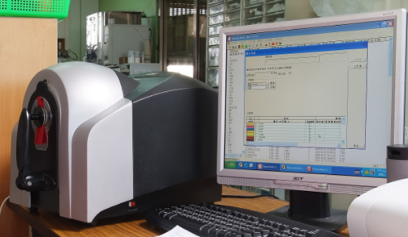
\includegraphics[width=8cm, height=5cm]{Graph/datacolor.png}
\caption{Datacolor MATCH儀器}
\label{fig:datacolor}
\end{figure}
就染整工廠的現況,基本上是依照工廠內工程師的經驗來做為調控製程參數的依據,一般都是以現有或過去的習慣而歸納出的製程參數,再由Datacolor MATCH所建議的染色配方及過往所設定的製程參數,在實驗室做少量的打樣實作。一般染整工廠在化驗室中如圖\ref{fig:factory}(左圖)為經過實驗而放置不同顏色的染料溶液,再將5公克的布根據設定的顏色進行打樣,再由驗色機去檢測與實際需求的差異是否在允許的範圍內。如果差異過大,則工程師必須回到配方設計的步驟進行調整,並且也將此數據輸入至Datacolor MATCH內的資料庫,做為爾後配方數據的修正資料。如驗色機檢測出之差異值在允許範圍內,則實際量產染色布料,就會將300到600公斤的布料放進大染缸內進行大量的染色,如圖\ref{fig:factory}(右圖)為工廠內部的大染缸
\begin{figure}[!htbp]
\centering
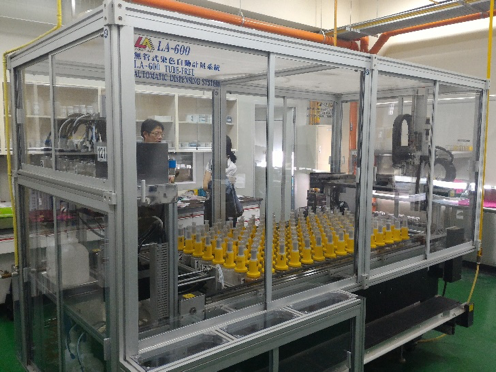
\includegraphics[width=7cm, height=5cm]{Graph/lab.png}
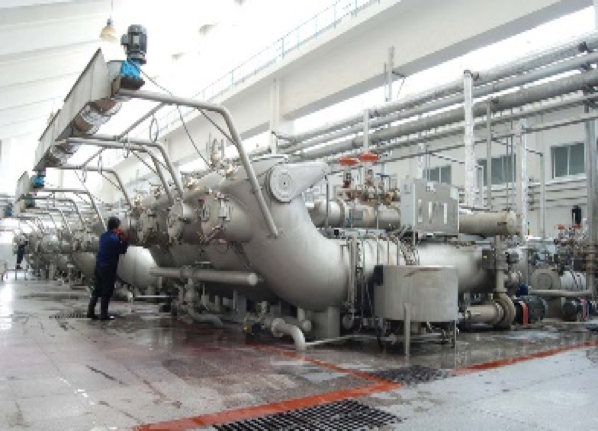
\includegraphics[width=7cm, height=5cm]{Graph/process.png}
\caption{化驗室以及染色工廠大染缸}
\label{fig:factory}
\end{figure}
。假如量產結果出現顏色異常,就必須回到打樣驗色步驟進行調整,現有的實驗室染整工廠的製程現況以圖~\ref{fig:flow2}表示。
\begin{figure} 
\centering
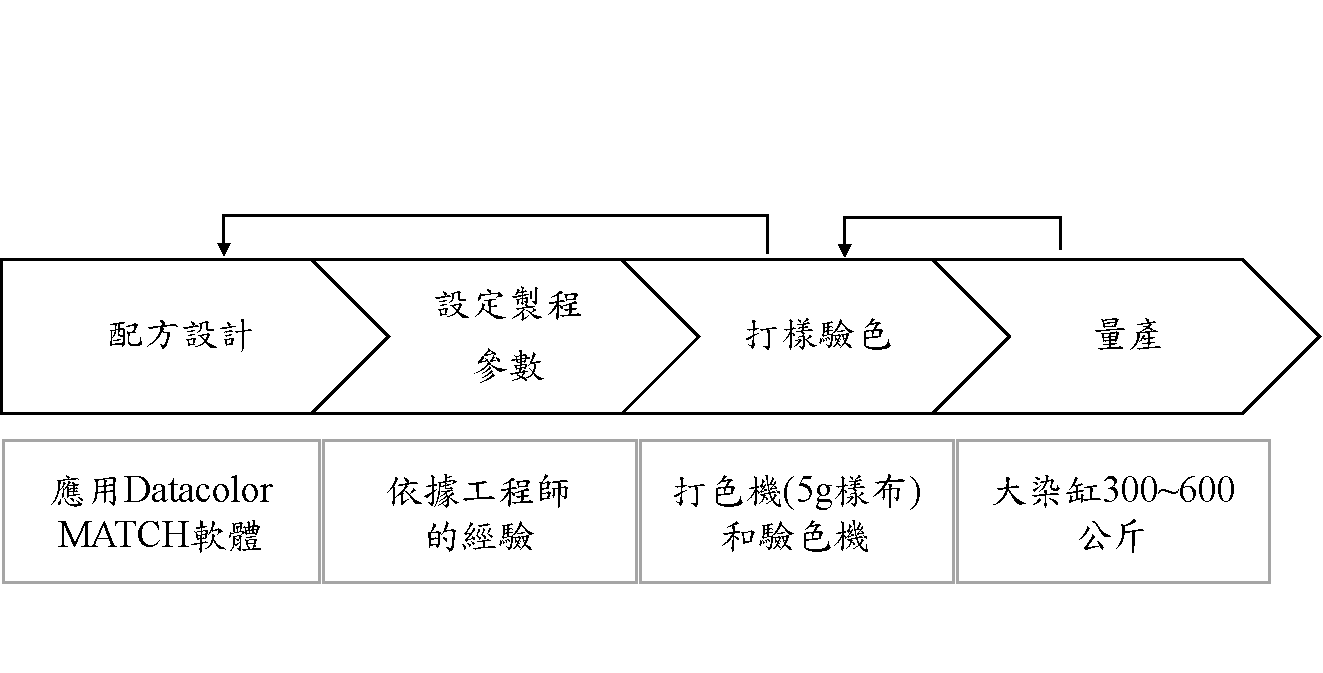
\includegraphics[width=14cm, height=6.5cm]{Graph/flowChart2.pdf}
\caption{染整工廠製程現況}
\label{fig:flow2}
\end{figure}
紡織業者除了以$\Delta E$作為布料染色品質的依據外,還有色力度($K/S$)也同樣作為品質考量的依據之一,色力度值同樣也是由Datacolor MATCH軟體所能檢測的結果之一,其主要檢測的目標是對布料染色後與客戶所要求的布料顏色間的深淺程度是否有一致,通常如果為一致,則色力度會為100,而通常人眼能辨識的差異在於正負5個單位,如果超出範圍就會需要重新染色或是報廢處理。

由以上所述,染整工廠的製程步驟中,製程參數的設定,基本上是依照工廠內工程師的經驗來做為調控製程參數的依據,再以Datacolor MATCH所建議的染色配方做為打樣驗色及量產的配方。然而,依照經驗所設定的製程參數,可能會有下列的情況:
\begin{enumerate}[(1)]
	\item 製程參數的設定會影響生產成本的高低:製程參數包括染整各階段的升溫速率、持溫時間,降溫溫度,製程參數的設定會影響染整過程所耗用的能源費用。
	\item 製程參數的設定會影響品質成本的高低:過往製程參數的經驗值有可能是落在製程參數的敏感區域,就是如果製程參數只是稍微變動,可能對染色表現因子(如色差值$\Delta E$或固色力)有很大的影響。
\end{enumerate}
